\documentclass{article}
\usepackage[margin=2cm]{geometry}
\usepackage[utf8]{inputenc}
\usepackage{amsfonts}
\usepackage{amsmath}
\usepackage{multicol}
\usepackage{amsthm}
\usepackage{amssymb}
\usepackage{graphicx}
\newtheorem{theorem}{Theorem}[section]
\newtheorem{corollary}{Corollary}[theorem]
\newtheorem{lemma}[theorem]{Lemma}
\title{Homework Set 1}
\author{Warren Atkison}
\date{\today}
\begin{document}

\maketitle

\section*{From the Reading}
\subsection*{Problem 4}
There was a time at which the study of dynamics languished, but for two notable exceptions: 
\paragraph*{}
One was the work of the french mathematicians Pierre Fatou and Gaston Julia in the 1920's on the dynamics of complex analytical maps. The second was the American mathematician G. D. Birkhoff who adopted Poincare's qualitative point of view on dynamics 
\subsection*{Problem 7}
Estimate $\sqrt{7}$ using the Babylonian algorithm given in Chapter 2. Use $x_0 = 2$ and compute $x_1,x_2,x_3,x_4$ keeping at least 6 digits.
\[
	x_{i+1} = \frac{1}{2}\left(x_i + \frac{7}{x_i}\right)
\]
\begin{align*}
	x_1 &= \frac{1}{2}\left(2 + \frac{7}{2}\right) = 2.75 \\
	x_2 &= \frac{1}{2}\left(2.75 + \frac{7}{2.75}\right) = 2.64773 \\
	x_3 &= \frac{1}{2}\left(2.6477 + \frac{7}{2.6477}\right) = 2.64575 \\
	x_4 &= \frac{1}{2}\left(2.64575 + \frac{7}{2.64575}\right) = 2.64575
\end{align*}
\section*{Sequences, Limits and Convergence}
\subsection*{Problem 3}
Find the limit of each sequence (you may assume convergence)
\begin{itemize}
	\item[(a)] $a_{n+1} = 1/(1+a_n)$ \\
	Let $L$ be the limit of the sequence, so that
	\begin{align*}
		\lim_{n \to \infty} a_n &= L & \lim_{n \to \infty} a_{n+1} = L
	\end{align*}
	Then
	\[
		L = 1/(1+L) \implies L(1+L) - 1 = 0 \implies L^2 + L - 1 = 0 \implies L = \frac{-1 \pm \sqrt{5}}{2}
	\]
	Both solutions work.
	\item[(b)] $a_{n+1} = \frac{1}{2}(a_n + 6)$ \\
	Let $L$ be the limit of the sequence, so that
	\begin{align*}
		\lim_{n \to \infty} a_n &= L & \lim_{n \to \infty} a_{n+1} = L
	\end{align*}
	Then
	\[
		L = \frac{1}{2}(L + 6) \implies L - 6 = 0 \implies L = 6
	\]
\end{itemize}	
\section*{Chapter 3}
\subsection*{Exercise 7}
Find all real fixed points (if any) for each of the following functions:
\begin{itemize}
	\item[b.] $F(x) = x^2 - 2$
		\begin{align*}
			x &= x^2 - 2 \implies x^2 - x - 2 = 0 \implies x = \frac{1 \pm 3}{2}
		\end{align*}
	\item[d.] $F(x) = x^3 - 3x$	
		\begin{align*}
			x &= x^3 - 3x \implies x(x^2 - 4) = 0 \implies x = 0,2,-2
		\end{align*}
\end{itemize}
\subsection*{Exercise 10}
Consider the functions $F(x) = |x - 2|$
\begin{itemize}
	\item[a.] What are the fixed points for $F$?
		\[
			x = |x - 2| \implies |x - 2| - x = 0 \implies x = 1
		\]
	\item[b.] If $m$ is an odd integer, what can you say about the orbit of $m$?
		\paragraph*{}
		The orbit is eventually fixed. $m$ converges to 1
	\item[c.] What happens to the orbit if $m$ is even?
		\paragraph*{}
		The orbit is eventually periodic. $m$ converges to a 2-cycle of $2,-2$
\end{itemize}
\subsection*{The Computer May Lie}
Consider the following function
\[
	D(x) = \begin{cases}
		2x & 0\leq x < 1/2 \\
		2x -1 & 1/2 \leq x < 1
	\end{cases} 
\]
Choose 10 initial seeds on the interval $(0,1)$. Compute the first 200 points on the corresponding orbit and record the results. Does the computer agree with what we know about certain orbits or does it give false results? Explain why the computer may lie. 
\begin{itemize}
	\item[1.] $x_0 = 1/9$ \\
		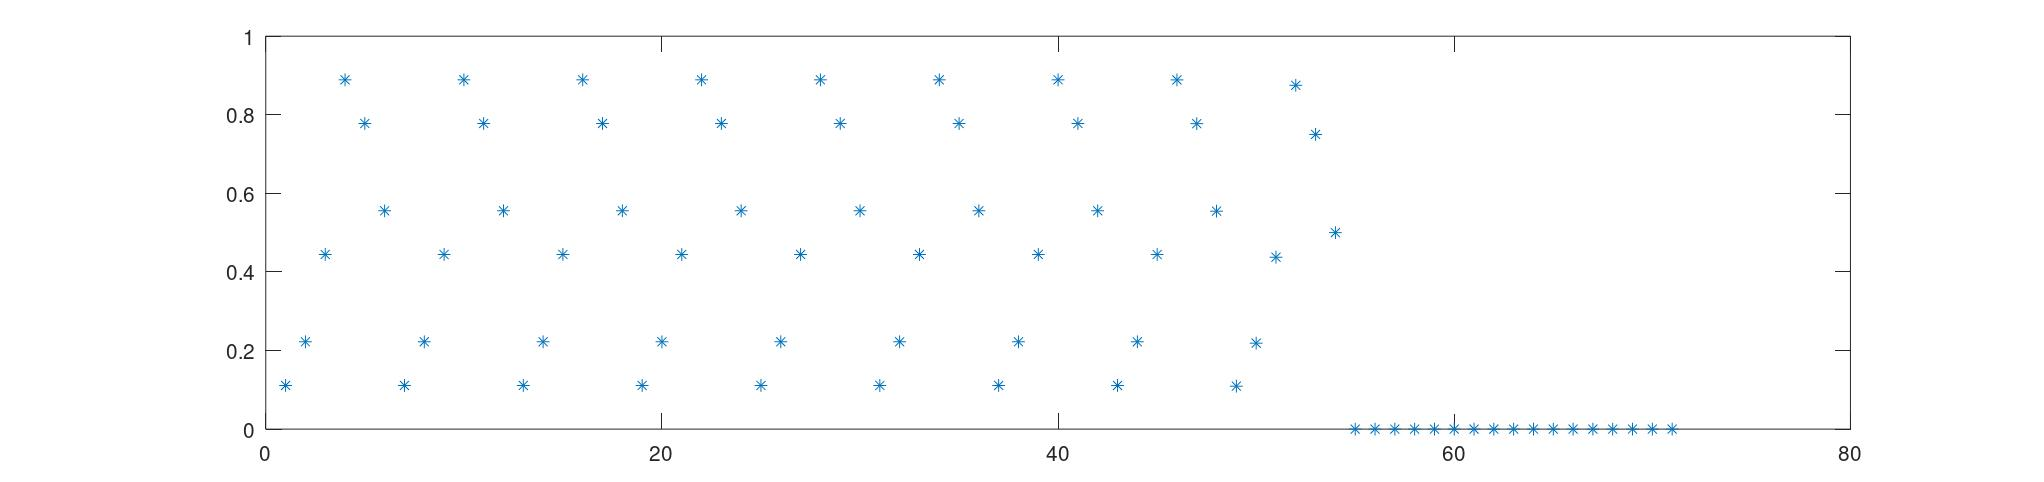
\includegraphics[scale = 0.2]{Fig1.3.6.1.jpg}
	\item[2.] $x_0 = 1/8$ \\
		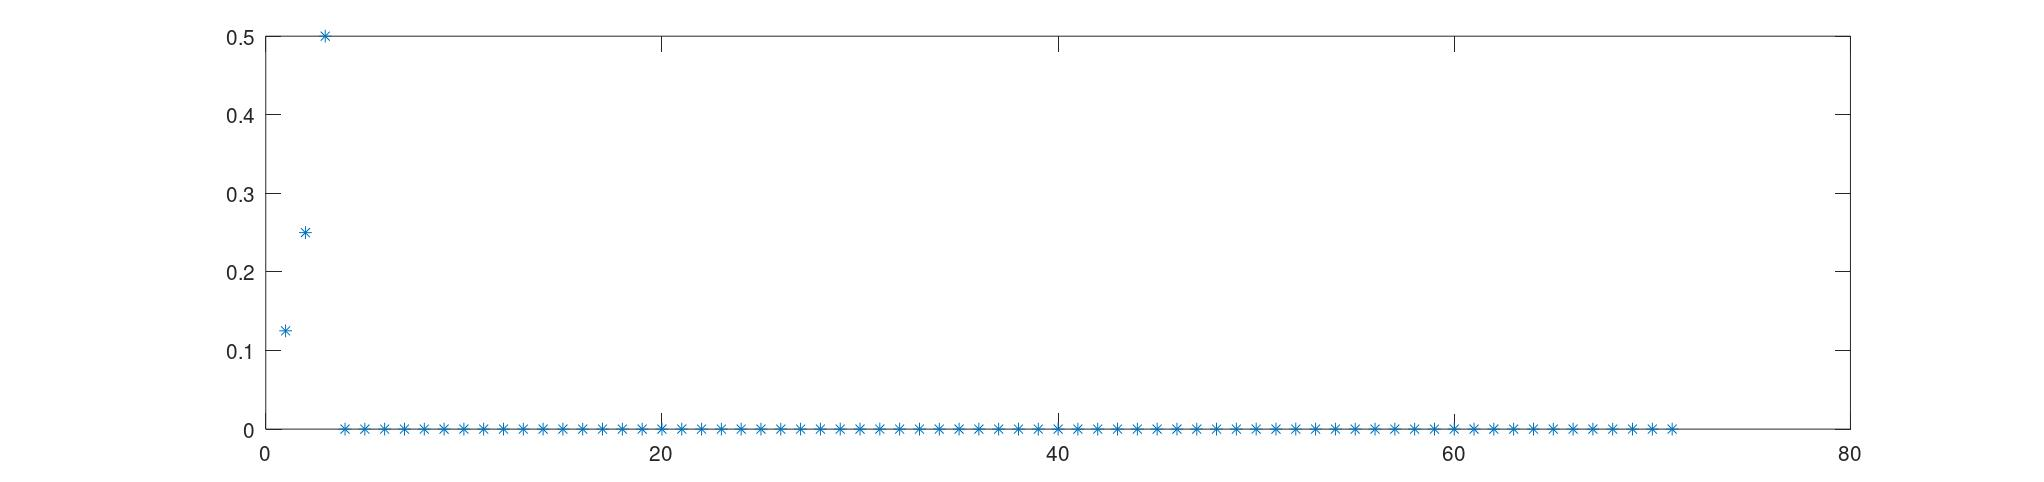
\includegraphics[scale = 0.2]{Fig1.3.6.2.jpg}
	\item[3.] $x_0 = 1/7$ \\
		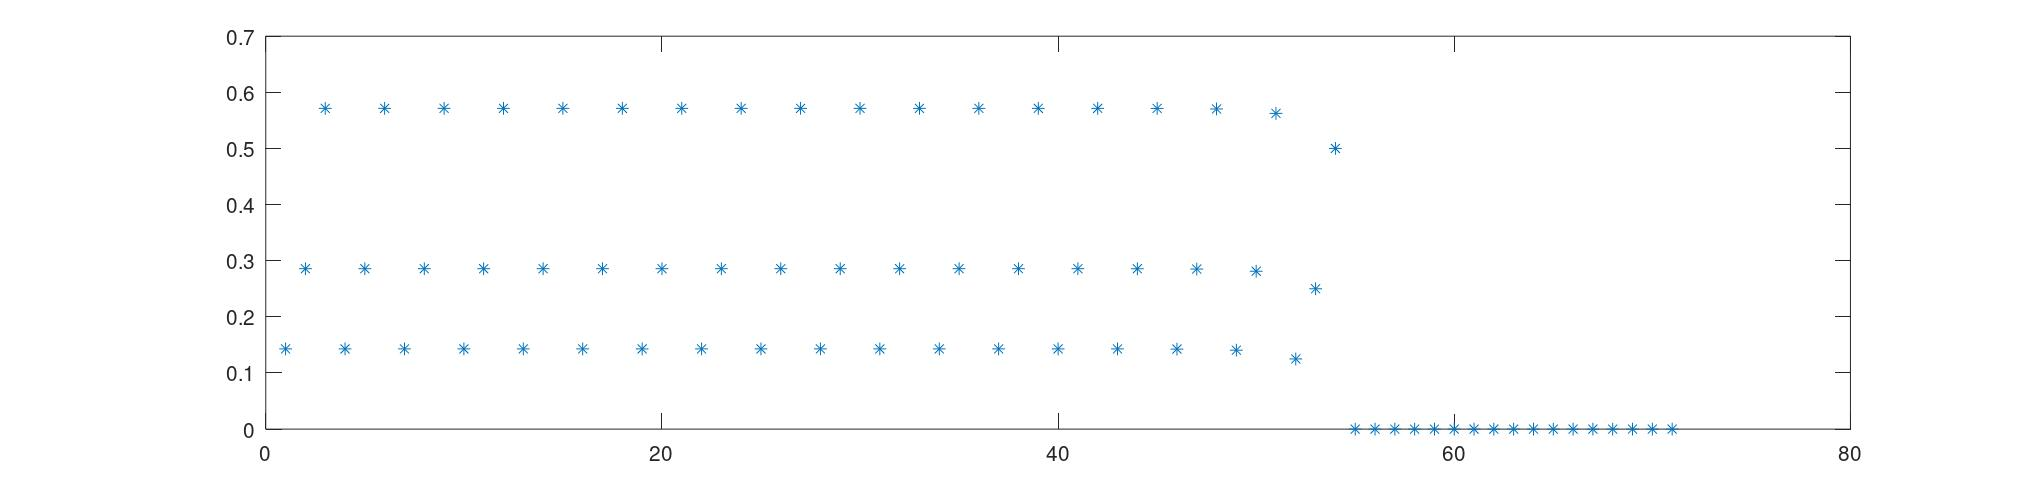
\includegraphics[scale = 0.2]{Fig1.3.6.3.jpg}
	\item[4.] $x_0 = 1/6$ \\
		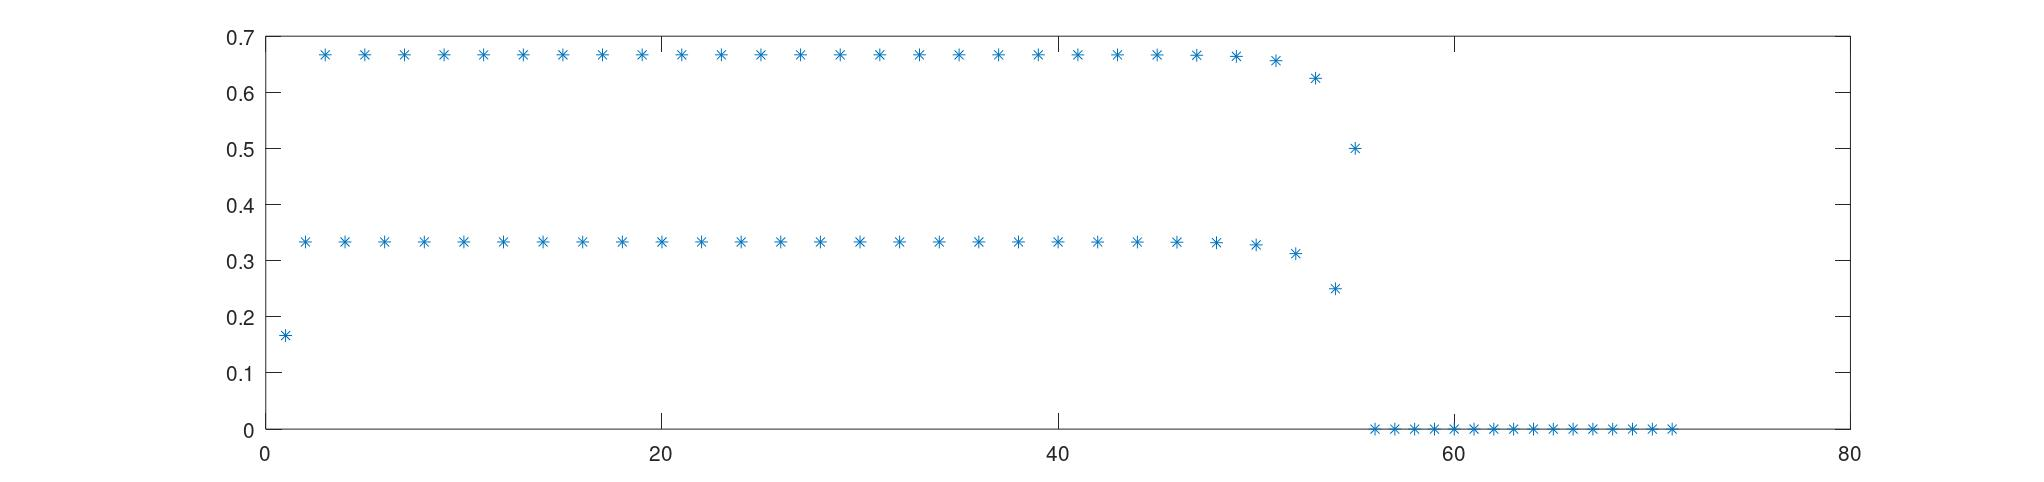
\includegraphics[scale = 0.2]{Fig1.3.6.4.jpg}
	\item[5.] $x_0 = 1/5$ \\
		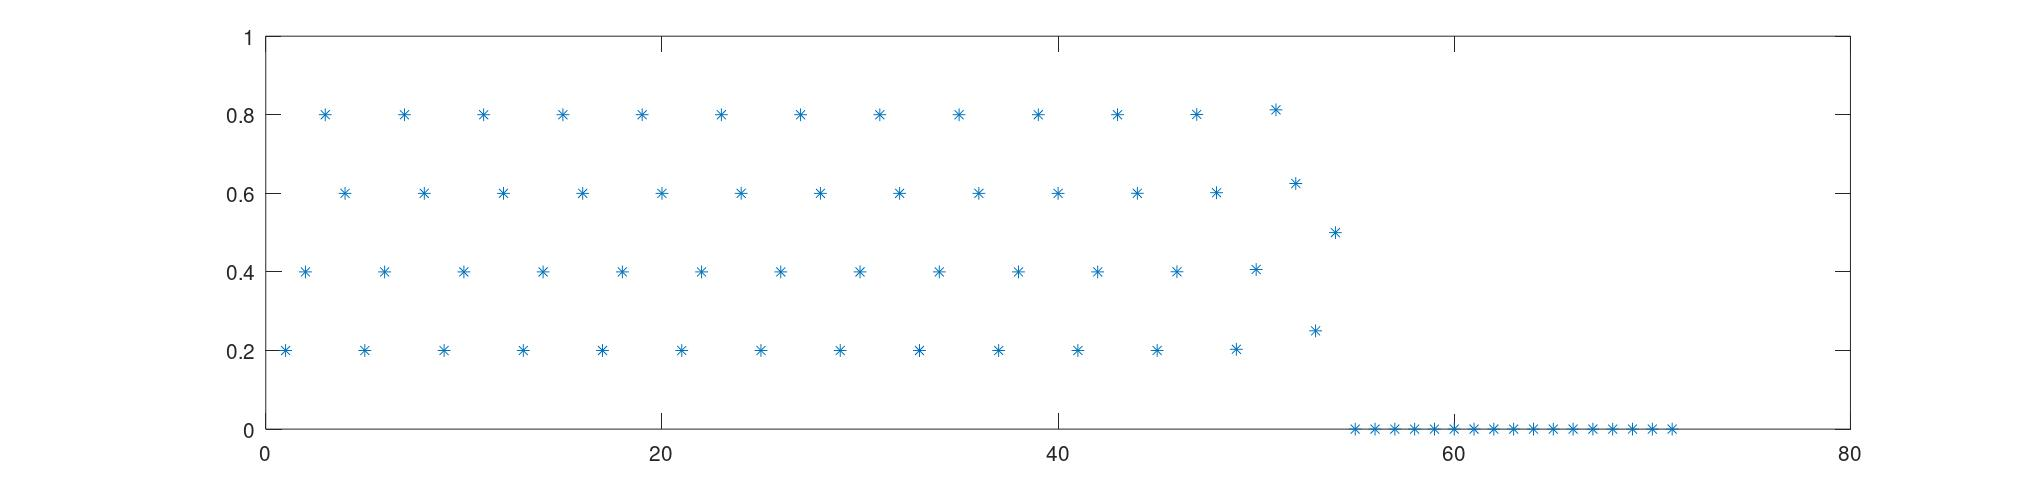
\includegraphics[scale = 0.2]{Fig1.3.6.5.jpg}	
	\item[6.] $x_0 = 1/4$ \\
		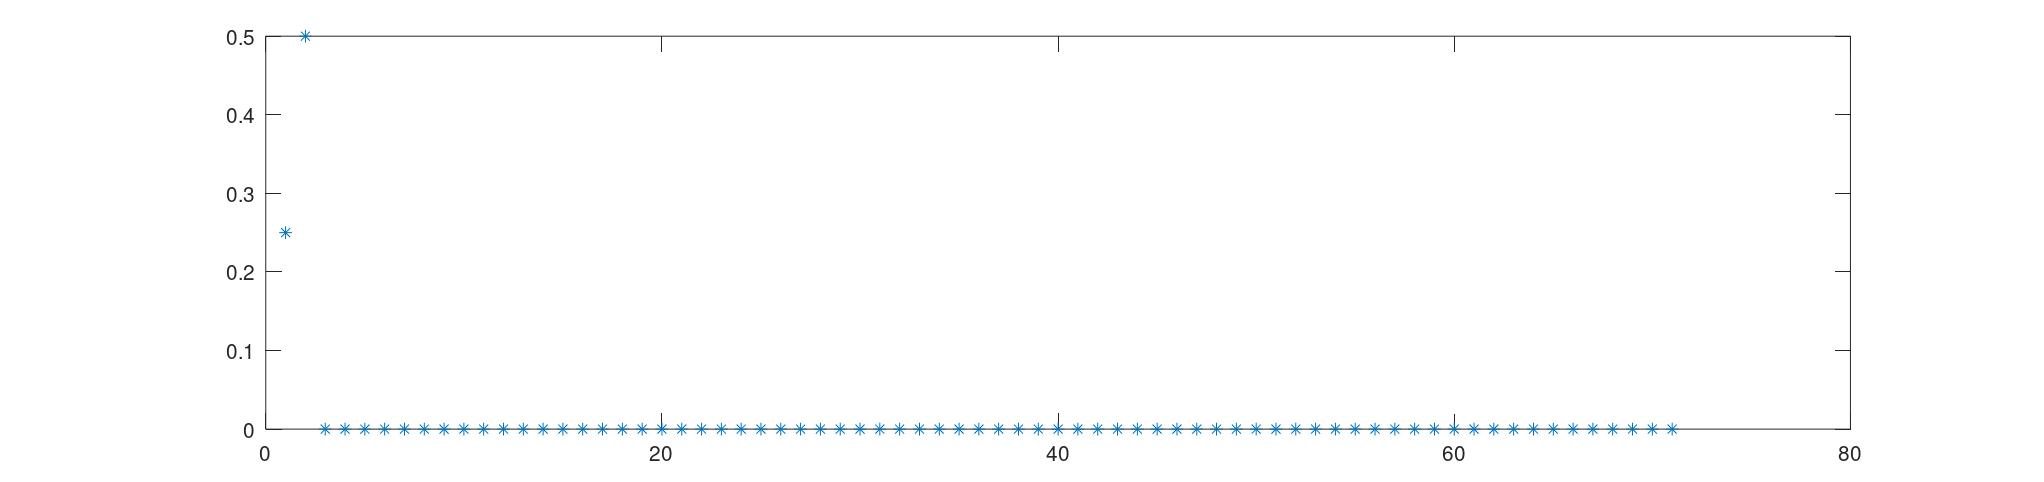
\includegraphics[scale = 0.2]{Fig1.3.6.6.jpg}
	\item[7.] $x_0 = 1/3$ \\
		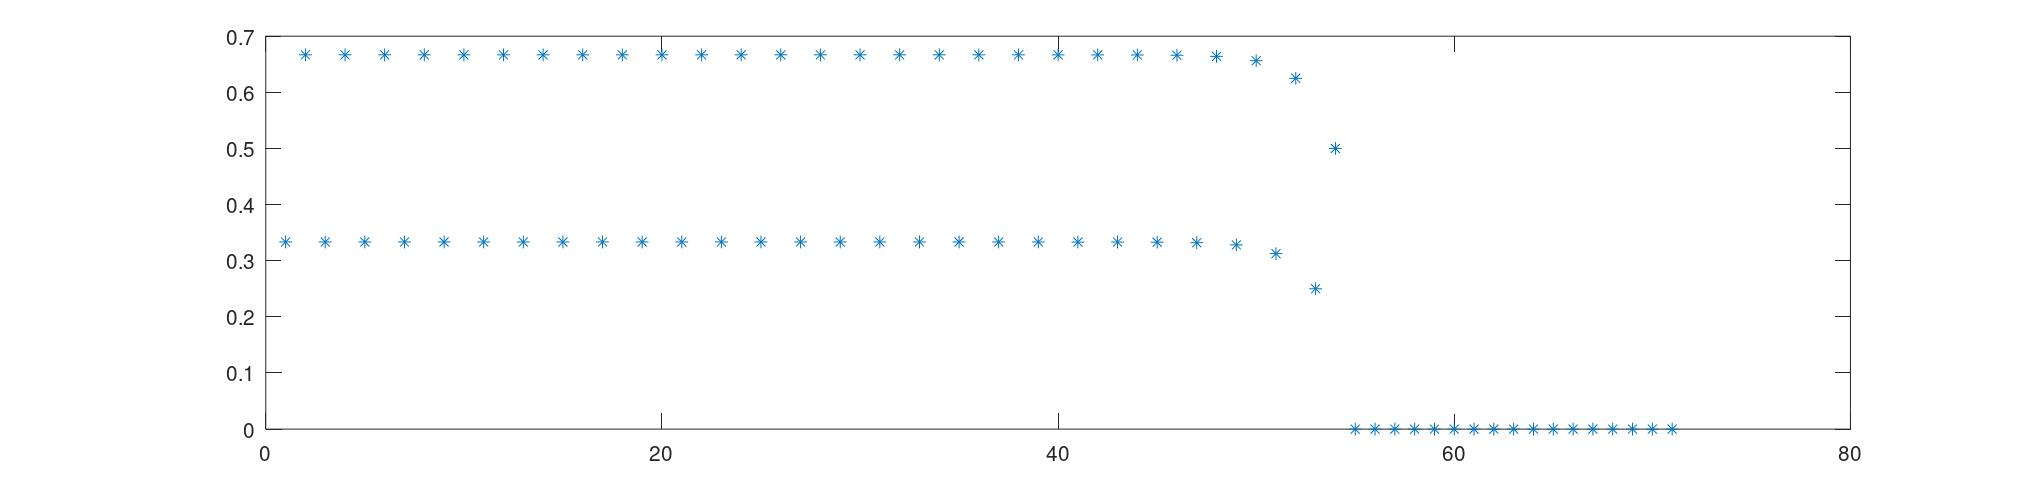
\includegraphics[scale = 0.2]{Fig1.3.6.7.jpg}
	\item[8.] $x_0 = 1/2$ \\
		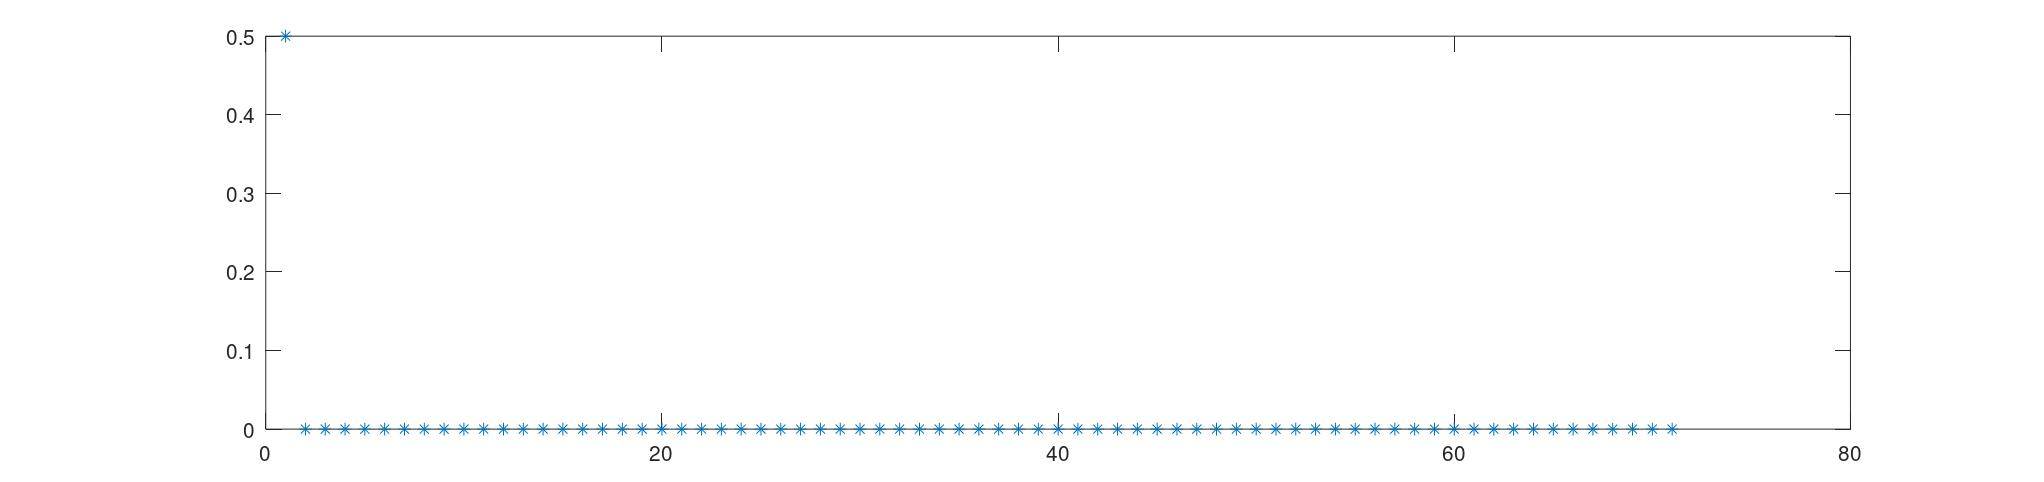
\includegraphics[scale = 0.2]{Fig1.3.6.8.jpg}	
	\item[9.] $x_0 = 2/3$ \\
		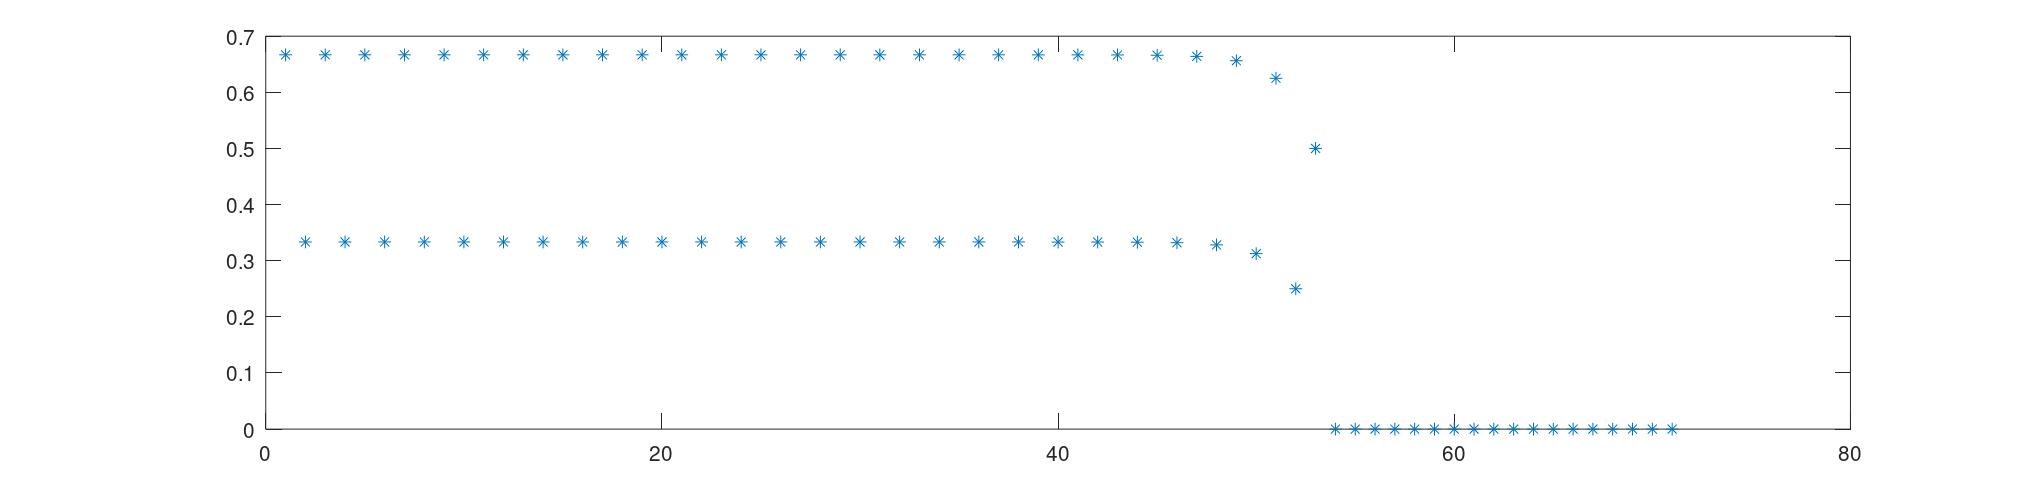
\includegraphics[scale = 0.2]{Fig1.3.6.9.jpg}	
	\item[10.] $x_0 = 3/8$ \\
		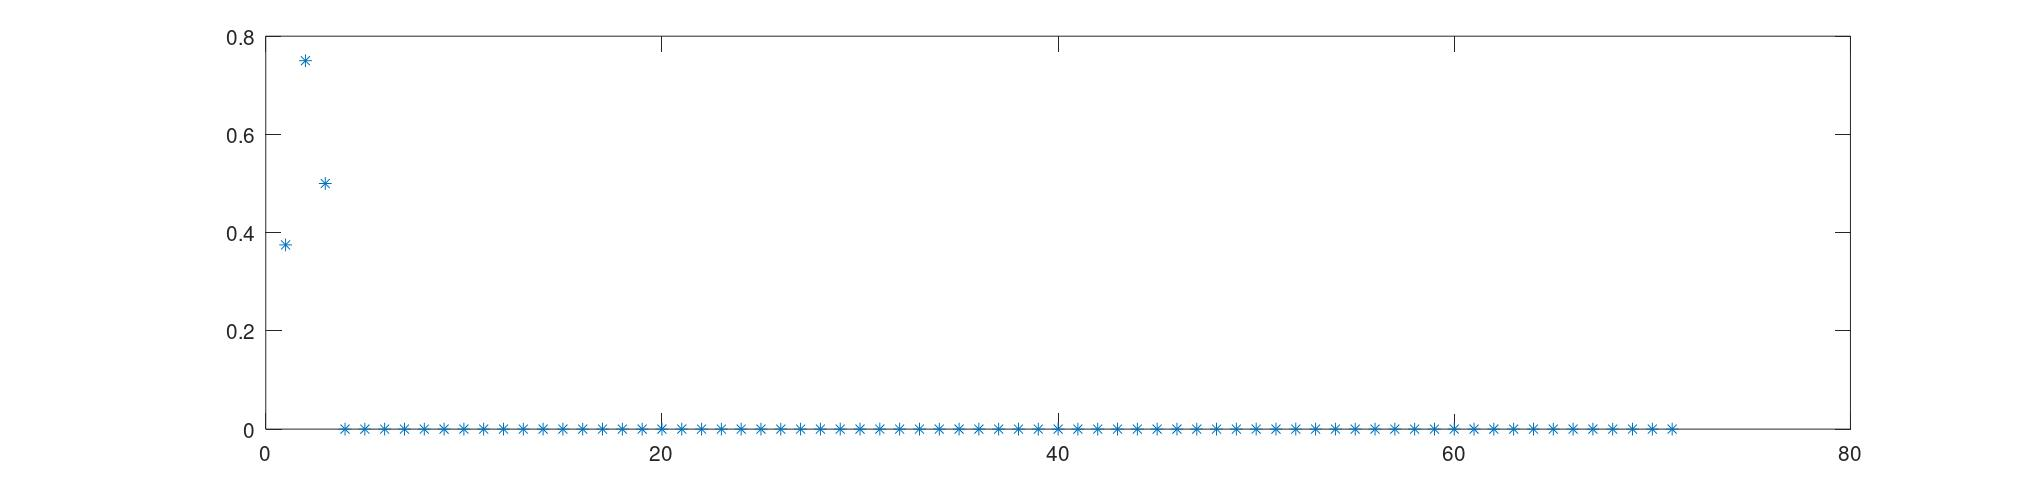
\includegraphics[scale = 0.2]{Fig1.3.6.10.jpg}	
\end{itemize}
\paragraph*{}
The only time the computer is correct is when $x_0$ is eventually fixed, as we can see with $1/2$, $1/4$, $1/8$, $3/8$. However, when $x_0$ is eventually periodic, the computer does some weird things. For the first 50 or so iterations the computer has no problem cycling through the orbit, but at some point the computer collapses the sequence down to 0.  
\paragraph*{}
As the textbook suggests, this may occur due to the fact that these numbers are stored as a finite sum and it's only an approximation. The sum is
\[
	\frac{a_1}{2} + \frac{a_2}{2^2} + \cdots + \frac{a_n}{2^n}
\]
As we can see with $1/2$, $1/4$, $1/8$, and $3/8$ these numbers that are of the form $\frac{m}{2^n}$ are all eventually fixed. We can conjecture that any number of the form $\frac{m}{2^n}$ is fixed for the doubling function and will go to 0. Then, the sum $\frac{a_1}{2} + \frac{a_2}{2^2} + \cdots + \frac{a_n}{2^n}$ is also of this form so any number stored into this form is eventually fixed, which is why we see every point simulated go to 0.


\end{document}
